\chapter{Semiconductors: Making Silicon Useful}
\label{ch:semis}

A computer needs billions of switches that can be flipped by an electrical signal, with no moving parts, billions of times per second. Metals cannot do this: they always conduct. Insulators cannot either: they never conduct. We need a material whose ability to conduct can be \emph{controlled}. That material is a semiconductor, almost always silicon. This chapter explains what makes silicon special, how ``doping'' turns it into a building material, and how temperature changes its behavior, which is one of the questions from the assessment.

\section{Electrons that can and cannot move}

Recall from Chapter~\ref{ch:electricity} that a material conducts when some of its electrons are free to move. Whether they are free depends on how tightly atoms hold their outermost electrons, called \term{valence electrons}.

\begin{itemize}
  \item In a \term{metal}, valence electrons are not tied to any one atom. They form a ``sea'' of free electrons that drifts easily when a voltage is applied. Metals conduct very well.
  \item In an \term{insulator}, every electron is locked in a chemical bond. Breaking one free takes a lot of energy, so almost none are free.
  \item In a \term{semiconductor}, electrons are bound, but not very tightly. A small amount of energy, such as heat at room temperature, frees a few of them.
\end{itemize}

Physicists describe this with an energy gap, the \term{band gap}: the minimum energy needed to free a bound electron. Silicon's band gap is about 1.12 electron-volts (eV). Silicon dioxide, a good insulator, has a gap of about 9\,eV. Metals have no gap at all.

\section{The silicon crystal}

A silicon atom has four valence electrons. In a crystal, each silicon atom shares one electron with each of four neighbors, forming four bonds (Figure~\ref{fig:silattice}). Every electron is used in a bond, so at very low temperature pure silicon is an insulator.

At room temperature, atoms vibrate. Occasionally the vibration shakes an electron out of its bond. Two things result:
\begin{enumerate}
  \item A \term{free electron} that can wander through the crystal and carry current.
  \item A \term{hole}: the empty spot where the electron used to be.
\end{enumerate}
In pure silicon at room temperature, fewer than one atom in a trillion has lost an electron this way, so pure silicon conducts very poorly.

\begin{figure}[h]
\centering
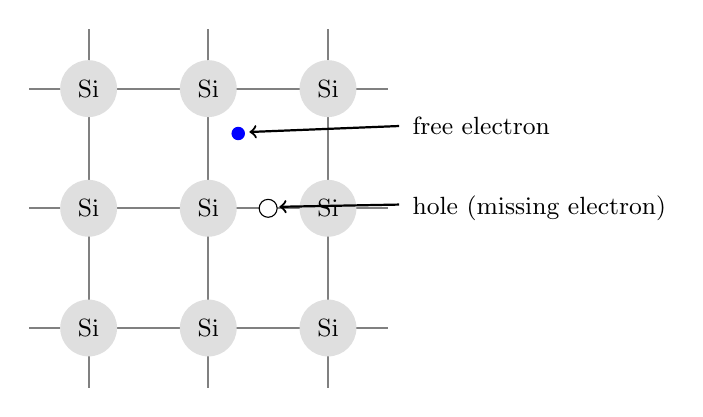
\begin{tikzpicture}[scale=0.95]
  \foreach \x in {0,1.6,3.2} \foreach \y in {0,1.6,3.2} {
    \draw[thick,gray] (\x,\y) -- ++(0.8,0); \draw[thick,gray] (\x,\y) -- ++(-0.8,0);
    \draw[thick,gray] (\x,\y) -- ++(0,0.8); \draw[thick,gray] (\x,\y) -- ++(0,-0.8);
    \fill[gray!25] (\x,\y) circle (0.38); \node at (\x,\y) {\small Si};}
  \fill[white] (2.4,1.6) circle (0.12); \draw (2.4,1.6) circle (0.12);
  \node[right,font=\small] at (4.2,1.6) {hole (missing electron)};
  \draw[->,thick] (4.15,1.65) -- (2.55,1.62);
  \fill[blue] (2.0,2.6) circle (0.09);
  \node[right,font=\small] at (4.2,2.7) {free electron};
  \draw[->,thick] (4.15,2.7) -- (2.15,2.62);
\end{tikzpicture}
\caption{Silicon atoms each share four bonds. Heat occasionally frees an electron, leaving a hole behind.}
\label{fig:silattice}
\end{figure}

\section{Holes: the missing electron that moves}

A hole is not a particle; it is the absence of an electron. But it behaves like a positive charge that can move. Here is why. If a neighboring bonded electron hops into the hole, the hole has effectively moved to where that electron came from. Under a voltage, electrons hop one way and the hole travels the other way, exactly as a positive charge would.

\begin{everyday}
Picture a row of full seats in a theater with one empty seat. When the person next to the empty seat slides over, the empty seat moves one place the other way. Keep sliding and the empty seat ``travels'' down the row, even though only people moved. The hole is the empty seat.
\end{everyday}

So a semiconductor has \emph{two} kinds of charge carriers: negative electrons and positive holes. This is the key to building two kinds of transistors.

\section{Doping: controlling the carriers}
\label{sec:doping}

Pure silicon has too few carriers to be useful. \term{Doping} adds a tiny, carefully controlled amount of another element, typically a few atoms per million or less, and changes conductivity enormously.

\paragraph{n-type silicon.} Add atoms with \emph{five} valence electrons, such as phosphorus or arsenic. Four electrons bond with silicon neighbors; the fifth has nothing to bond with and is freed easily. The silicon now has many free electrons, which carry negative charge, so it is called \term{n-type}. Electrons are its \term{majority carriers}; holes are \term{minority carriers}.

\paragraph{p-type silicon.} Add atoms with \emph{three} valence electrons, such as boron. One bond is left incomplete, creating a hole. The silicon now has many holes, which act as positive carriers, so it is called \term{p-type}. Holes are its majority carriers.

\begin{remember}
\textbf{n}-type: extra \textbf{n}egative carriers (electrons), from 5-electron dopants like phosphorus.\\
\textbf{p}-type: extra \textbf{p}ositive carriers (holes), from 3-electron dopants like boron.\\
A doped crystal is still electrically neutral overall: every extra free electron is balanced by a positive dopant nucleus, and every hole by a negative one.
\end{remember}

Chip designers write \term{n+} or \term{p+} for heavily doped regions (which conduct well and form transistor terminals), and speak of an \term{n-well}: a region of n-type silicon built into a p-type wafer so that both kinds of transistor can live on the same chip (Chapter~\ref{ch:mosfet}).

\section{How carriers move: drift, diffusion and mobility}

Carriers move for two reasons:
\begin{itemize}
  \item \term{Drift}: an electric field (a voltage across a distance) pushes them. Electrons drift toward the higher voltage; holes toward the lower.
  \item \term{Diffusion}: carriers spread from where they are crowded to where they are sparse, like a drop of ink spreading in water. No voltage is needed.
\end{itemize}

How fast a carrier drifts in a given field is its \term{mobility}, written $\mu$ (mu):
\[
  v_{\text{drift}} = \mu\,E,
\]
where $E$ is the electric field (volts per meter). Higher mobility means faster carriers, more current, and faster transistors.

\begin{center}
\begin{tabular}{ll}
\toprule
Carrier in silicon & Mobility (lightly doped, room temperature) \\
\midrule
Electrons & about 1400\,cm$^2$/(V$\cdot$s) \\
Holes & about 450\,cm$^2$/(V$\cdot$s) \\
\bottomrule
\end{tabular}
\end{center}

\begin{bigidea}
Electrons are about two to three times more mobile than holes. Holes move only by electrons hopping from bond to bond, which is slower than a free electron's travel. This single fact is why PMOS transistors (which use holes) are weaker than NMOS transistors (which use electrons), and why PMOS transistors are usually drawn about twice as wide (Chapter~\ref{ch:mosfet}).
\end{bigidea}

At very high fields, carriers stop speeding up; their velocity levels off at roughly $10^7$\,cm/s. This \term{velocity saturation} matters in modern, very short transistors.

\section{What heat does to semiconductors and to metal}
\label{sec:tempmobility}

Temperature changes conduction in two competing ways, and semiconductors and metals respond differently.

\paragraph{Effect 1: more scattering, so lower mobility.} A hotter crystal vibrates more. Carriers moving through it collide with the vibrating atoms more often (these vibrations are called \term{phonons}, and the collisions \term{phonon scattering}). More collisions mean carriers cannot build up speed, so \textbf{mobility decreases as temperature increases}. Transistors therefore carry less current and get slower.

\paragraph{Effect 2: more carriers.} Heat also frees more electrons from bonds. In pure silicon the number of free carriers rises very steeply (exponentially) with temperature. In a transistor that is supposed to be off, those extra carriers show up as \term{leakage current}, which grows rapidly when the chip is hot.

\paragraph{Metals.} A metal's free electrons are already all free; heat does not add more. Only effect 1 applies: more vibration means more scattering. So \textbf{metal resistance increases with temperature}. For copper, resistance rises by about 0.4\% per \textdegree C, so a wire 100\,\textdegree C hotter has roughly 40\% more resistance.

\begin{onoa}
A reported question asked how carrier mobility and wire resistance change when temperature increases. Answer: \textbf{carrier mobility decreases} (more phonon scattering), so transistors drive less current; \textbf{wire resistance increases} (also more scattering), so wires get slower. Both effects make the circuit slower at high temperature. Chapter~\ref{ch:pvt} adds one twist: the transistor's threshold voltage also drops when hot, which pushes the other way and, at low supply voltages, can win.
\end{onoa}

\section{The PN junction and the diode}
\label{sec:pn}

Something important happens where p-type and n-type silicon meet, a \term{PN junction}.

Near the boundary, free electrons from the n side diffuse into the p side and fill holes; holes from the p side diffuse into the n side. Carriers near the boundary cancel out, leaving a thin \term{depletion region} with no free carriers. The dopant atoms left behind are charged (positive on the n side, negative on the p side), creating a built-in electric field that stops further diffusion. The built-in voltage is a few tenths of a volt.

This structure is a \term{diode}, a one-way valve for current:
\begin{itemize}
  \item \term{Forward bias} (p side more positive than n side): the applied voltage fights the built-in barrier, the depletion region shrinks, and current flows easily once the voltage exceeds about 0.6--0.7\,V for silicon. Current grows exponentially with voltage:
  \[
    I = I_S\left(e^{V/V_T} - 1\right), \qquad V_T = \frac{kT}{q} \approx 26~\text{mV at room temperature}.
  \]
  \item \term{Reverse bias} (n side more positive): the barrier grows, the depletion region widens, and only a tiny leakage current flows. At a large enough reverse voltage the junction \term{breaks down} and conducts heavily.
\end{itemize}

\begin{center}
\begin{circuitikz}
  \draw (0,0) node[left]{anode (p)} to[D] (2.5,0) node[right]{cathode (n)};
  \node[font=\small] at (1.25,-0.8) {current flows easily from anode to cathode};
\end{circuitikz}
\end{center}

Diodes matter to a digital designer in three ways:
\begin{itemize}
  \item Every transistor's source and drain form PN junctions with the silicon beneath them. These junctions must always stay reverse biased, which is why the p-type body under NMOS transistors is tied to ground and the n-well under PMOS transistors is tied to the supply (Chapter~\ref{ch:mosfet}).
  \item Reverse-biased junctions leak a little, adding to leakage power.
  \item Diodes are deliberately added to protect circuits: from static electricity (ESD protection) and from charge collected during manufacturing (antenna diodes, Chapter~\ref{ch:fab}).
\end{itemize}

\section{Silicon dioxide: silicon's perfect partner}

Silicon has a lucky property: heat it in oxygen and it grows a layer of \term{silicon dioxide} (SiO$_2$), essentially glass, which is an excellent insulator and bonds cleanly to the silicon. A thin layer of insulator on silicon is exactly what a transistor's gate needs (next chapter). In the most advanced processes, the gate insulator is so thin that designers switched to materials with higher permittivity (``high-$k$'' dielectrics such as hafnium oxide), which give the same capacitance with a physically thicker, less leaky layer.

\section{Summary}

\begin{itemize}
  \item Semiconductors sit between conductors and insulators: a little energy frees their electrons.
  \item Freeing an electron leaves a hole, which behaves like a moving positive charge.
  \item Doping controls carriers: phosphorus or arsenic makes n-type (electrons); boron makes p-type (holes).
  \item Mobility measures how fast carriers drift. Electrons are 2--3 times more mobile than holes, so NMOS is stronger than PMOS.
  \item Heat lowers mobility (transistors slow down), raises metal resistance (wires slow down), and sharply raises leakage.
  \item A PN junction is a diode: it conducts in forward bias and blocks (with slight leakage) in reverse bias.
\end{itemize}

\section{Exercises}

\begin{enumerate}
  \item Why is pure silicon a poor conductor at room temperature?
  \item Which dopant makes n-type silicon, boron or phosphorus? Explain using valence electrons.
  \item What are the majority carriers in p-type silicon?
  \item Electron mobility is about three times hole mobility. Name one consequence for chip design.
  \item As temperature rises, what happens to (a) carrier mobility, (b) copper wire resistance, (c) transistor leakage current?
  \item True or false: a hole is a positively charged particle, like a proton, that moves through the crystal.
  \item A silicon diode has 0.7\,V across it with the p side positive. Is it conducting? What if the polarity is reversed?
  \item Why is the p-type body under NMOS transistors connected to ground?
\end{enumerate}

\subsection*{Answers}
\begin{enumerate}
  \item All its valence electrons are locked in bonds; at room temperature heat frees only a tiny number, so there are very few carriers.
  \item Phosphorus. It has five valence electrons; four bond with silicon neighbors and the fifth is easily freed, adding free electrons.
  \item Holes.
  \item PMOS transistors are weaker for the same size, so they are made wider (about 2--3 times) to match NMOS strength; also, gate designs prefer to put PMOS in parallel rather than in series (Chapter~\ref{ch:cmos}).
  \item (a) Decreases. (b) Increases. (c) Increases, steeply.
  \item False. A hole is the absence of an electron in a bond. It behaves like a positive charge because neighboring electrons hop into it, making the vacancy move.
  \item Yes, it is forward biased and conducting. Reversed, it blocks current except for a tiny leakage.
  \item To keep the PN junctions between the n+ source/drain regions and the p-type body reverse biased (the body is at the lowest voltage), so they do not conduct.
\end{enumerate}
